% ------------------------------------------------------------------------
% ------------------------------------------------------------------------
% abnTeX2: Modelo de Trabalho Acadêmico em conformidade com 
% as normas da ABNT
% ------------------------------------------------------------------------
% ------------------------------------------------------------------------

\documentclass[english, 
               brazil, 
               msc] %Opções bsc (TCC) e msc (Mestrado)
               {dcomp-abntex2}

% Geração de dummy text
% Retirar para a versão final do documento
\usepackage{lipsum}


%Compila o indice
\makeindex

\begin{document}

% Seleciona o idioma do documento (conforme pacotes do babel)
\selectlanguage{brazil}

% Retira espaço extra obsoleto entre as frases.
\frenchspacing 

% ----------------------------------------------------------
% ELEMENTOS PRÉ-TEXTUAIS
% ----------------------------------------------------------
\pretextual

\titulo{Modelo Canônico de Trabalho Acadêmico com \abnTeX: Customização para o Departamento de Computação}
\autor{Arnold Schwarzenegger da Silva}
\orientador{Andrew S. Tanenbaum}
\coorientador{Donald Knuth}
\curso{Ciência da Computação}

\imprimircapa
\imprimirfolhaderosto*

   
\begin{dedicatoria}
   \vspace*{\fill}
   \centering
   \noindent
   \textit{I dedicate this thesis to all my family, friends and \\ 
   professors who gave me the necessary support to get here.} \vspace*{\fill}
\end{dedicatoria}
% ---
\begin{agradecimentos}

\lipsum[1-4]

\end{agradecimentos}
% ---
\begin{epigrafe}[]
    \vspace*{\fill}
	\begin{flushright}
	
		\textit{Este trabalho, além de cultural, filosófico e pedagógico\\
				É também medicinal, preventivo e curativo\\
				Servindo entre outras coisas para pano branco e pano preto\\
				Curuba e ferida braba\\
				Piolho, chulé e caspa\\
				Cravo, espinha e berruga\\
				Panarismo e água na pleura\\
				Só não cura o velho chifre\\
				Por que não mata a raiz\\
				Pois fica ela encravada\\
				No fundo do coração\\
				(Falcão)}
		
	\end{flushright}
\end{epigrafe}
% ---
% resumo em português
\setlength{\absparsep}{18pt} % ajusta o espaçamento dos parágrafos do resumo
\begin{resumo}
 
Segundo a \citeonline[3.1-3.2]{NBR6028:2003}, o resumo deve ressaltar o objetivo, o método, os resultados e as conclusões do documento. A ordem e a extensão destes itens dependem do tipo de resumo (informativo ou indicativo) e do tratamento que cada item recebe no documento original. O resumo deve ser precedido da referência do documento, com exceção do resumo inserido no próprio documento. (\ldots) As palavras-chave devem figurar logo abaixo do resumo, antecedidas da expressão Palavras-chave:, separadas entre si por ponto e finalizadas também por ponto.

 \textbf{Palavras-chave}: latex. abntex. editoração de texto.
\end{resumo}
% resumo em inglês
\setlength{\absparsep}{18pt} % ajusta o espaçamento dos parágrafos do resumo
\begin{resumo}[Abstract]
 \begin{otherlanguage*}{english}
   
The daily practice proves that the expansion of world markets can no longer be dissociated from the communication process as a whole. All these questions, properly considered, raise questions about the need for procedural renovation has not yet demonstrated convincingly that will participate in the change of the various schools of thought. The accumulated experience shows that the adoption of decentralization policies entails a process of reform and modernization of new propositions. 

I would like to emphasize that the clear definition of objectives presents trends in order to approve the maintenance of the undeniably appropriate conditions. Care to identify critical points in increasing the dialogue between the different productive sectors may prove to emphasize the relativity of information flow. Thinking longer term, the complexity of the studies conducted ensures the contribution of an important group in determining the general participation system. What we must always keep in mind is that the revolution of morals extends the reach and the importance of rules of conduct regulations. Moreover, the consolidation of the structures is an aperture for improving the budget sector. 

It is clear that the mobility of international capital points to improve the development guidelines for the future. Of course, the continued development of different forms of performance requires precision and defining the lifting of the variables involved. 

We can already glimpse the way the clear definition of objectives is an opening for the improvement of the various schools of thought. Care to identify critical points in need of renovation procedural encourages standardization of corporate paradigms. The daily practice proves that the beginning of the general activity of forming attitudes ensures the contribution of an important group in determining the expected long-term return. The accumulated experience shows that the hegemony of the political environment presents trends in order to approve the maintenance of rules of conduct regulations. 

Thus, the revolution of customs positively affects the correct prediction of the preferred directions towards progress. Therefore, a clear definition of objectives helps the preparation and composition of the methods used in evaluating results. The certification methodologies that help us cope with the impartial judgment of eventualities presents trends in order to approve the maintenance of vertical relationships between the hierarchies.
 
   \textbf{Keywords}: Algorithms, DataBase, Cloud Computing, Lero-Lero.
 \end{otherlanguage*}
\end{resumo}
    
% Lista de ilustrações
\pdfbookmark[0]{\listfigurename}{lof}
\listoffigures*
\cleardoublepage

% Lista de quadros
\pdfbookmark[0]{\listofquadrosname}{loq}
\listofquadros*
\cleardoublepage

% Lista de tabelas
\pdfbookmark[0]{\listtablename}{lot}
\listoftables*
\cleardoublepage

% Lista de códigos
\pdfbookmark[0]{\listlistingname}{lol}
\begin{KeepFromToc}
	\listoflistings
\end{KeepFromToc}
\cleardoublepage
   
% ---
% inserir lista de abreviaturas e siglas
% ---

\begin{siglas}
	\item[ABNT]{Associação Brasileira de Normas Técnicas}
	\item[abnTeX]{ABsurdas Normas para TeX}
  	\item[AFM]{Alphabet Frequency Matrix}
	\item[API]{Application Programming Interface}
	\item[ARIMA]{Auto-Regressive Integrated Moving Average}
	\item[BRN]{Bug Report Network}
	\item[BTS]{Bug Triage System}
	\item[CAS]{Context-Aware Systems}
	\item[CCB]{Change Control Board}
	\item[CR]{Change Request}
	\item[CVS]{Concurrent Version System}
	\item[ES]{Expert System}
	\item[FLOSS]{Free/Libre Open Source Software}
	\item[GLR]{Generalized Linear Regression}
	\item[GQM]{Goal Question Metric}
	\item[HTML]{HyperText Markup Language}
	\item[IR]{Information Retrieval}
	\item[IRT]{Recôncavo Institute of Technology}
	\item[JDT]{Jazz Duplicate Finder}
	\item[LDA]{Latent Dirichlet Allocation}
	\item[LOC]{Lines of Code}
	\item[LSI]{Latent Semantic Indexing}
	\item[MS]{Mapping Study}
	\item[MSR]{Mining Software Repositories}
	\item[NLP]{Natural Language Processing}
	\item[PROMISE]{Predictive Models in Software Engineering}
	\item[RBES]{Rule-Based Expert System}
	\item[RHEL]{RedHat Enterprise Linux}
	\item[SaaS]{Software as a Service}
	\item[SCM]{Software Configuration Management}
	\item[SERPRO]{Brazilian Federal Organization for Data Processing}
	\item[SLR]{Stepwise Linear Regression}
	\item[SLR]{Systematic Literature Review}
	\item[SVD]{Singular Value Decomposition}
	\item[SVM]{Support Vector Machine}
	\item[SVN]{Subversion}
	\item[TF-IDF]{Term Frequency-Inverse Document Frequency}
	\item[VSM]{Vector Space Model}
	\item[XP]{Extreming Programming}
\end{siglas}
% ---
% ---
% inserir lista de símbolos
% ---

\begin{simbolos}
  \item[$ \Gamma $] Letra grega Gama
  \item[$ \Lambda $] Lambda
  \item[$ \zeta $] Letra grega minúscula zeta
  \item[$ \in $] Pertence
\end{simbolos}
% ---
    
\pdfbookmark[0]{\contentsname}{toc}
\tableofcontents*
\cleardoublepage

% ----------------------------------------------------------
% ELEMENTOS TEXTUAIS
% ----------------------------------------------------------
\textual
\chapter{Introdução}

Nunca é demais lembrar o peso e o significado destes problemas, uma vez que a consolidação das estruturas é uma das consequências dos conhecimentos estratégicos para atingir a excelência. Não obstante, a contínua expansão de nossa atividade causa impacto indireto na reavaliação das posturas dos órgãos dirigentes com relação às suas atribuições. As experiências acumuladas demonstram que o aumento do diálogo entre os diferentes setores produtivos representa uma abertura para a melhoria do processo de comunicação como um todo. Evidentemente, o surgimento do comércio virtual prepara-nos para enfrentar situações atípicas decorrentes das direções preferenciais no sentido do progresso. A certificação de metodologias que nos auxiliam a lidar com a percepção das dificuldades facilita a criação dos modos de operação convencionais. 

O cuidado em identificar pontos críticos no comprometimento entre as equipes cumpre um papel essencial na formulação do retorno esperado a longo prazo.

\section{AbnTeX2}
Este documento e seu código-fonte são exemplos de referência de uso da classe
\emph{abntex2} e do pacote \emph{abntex2cite}. O documento 
exemplifica a elaboração de trabalho acadêmico (tese, dissertação e outros do
gênero) produzido conforme a ABNT NBR 14724:2011 \emph{Informação e documentação
- Trabalhos acadêmicos - Apresentação}.

A expressão ``Modelo Canônico'' é utilizada para indicar que \abnTeX\ não é
modelo específico de nenhuma universidade ou instituição, mas que implementa tão
somente os requisitos das normas da ABNT. Uma lista completa das normas
observadas pelo \abnTeX\ é apresentada em \citeonline{abntex2classe}.

Sinta-se convidado a participar do projeto \abnTeX! Acesse o site do projeto em
\url{http://www.abntex.net.br/}. Também fique livre para conhecer,
estudar, alterar e redistribuir o trabalho do \abnTeX, desde que os arquivos
modificados tenham seus nomes alterados e que os créditos sejam dados aos
autores originais, nos termos da ``The \LaTeX\ Project Public
License''\footnote{\url{http://www.latex-project.org/lppl.txt}}.

Encorajamos que sejam realizadas customizações específicas deste exemplo para
universidades e outras instituições --- como capas, folha de aprovação, etc.
Porém, recomendamos que ao invés de se alterar diretamente os arquivos do
\abnTeX, distribua-se arquivos com as respectivas customizações.
Isso permite que futuras versões do \abnTeX~não se tornem automaticamente
incompatíveis com as customizações promovidas. Consulte
\citeonline{abntex2-wiki-como-customizar} par mais informações.

Este documento deve ser utilizado como complemento dos manuais do \abnTeX\ \cite{abntex2classe,abntex2cite,abntex2cite-alf} e da classe \emph{memoir \cite{memoir}}. 

Esperamos, sinceramente, que o \abnTeX\ aprimore a qualidade do trabalho que
você produzirá, de modo que o principal esforço seja concentrado no principal:
na contribuição científica.

Equipe \abnTeX 

Lauro César Araujo

\section{Estratégias em um Novo Paradigma Globalizado}
Por conseguinte, a contínua expansão de nossa atividade apresenta tendências no sentido de aprovar a manutenção das posturas dos órgãos dirigentes com relação às suas atribuições. Por outro lado, a hegemonia do ambiente político exige a precisão e a definição do impacto na agilidade decisória. No mundo atual, o desafiador cenário globalizado facilita a criação das direções preferenciais no sentido do progresso. No entanto, não podemos esquecer que o entendimento das metas propostas estende o alcance e a importância das condições financeiras e administrativas exigidas. Pensando mais a longo prazo, a valorização de fatores subjetivos garante a contribuição de um grupo importante na determinação das regras de conduta normativas. 

\begin{lstlisting}[caption={Primeiro código Java},label=Java1, language=java]

public class HelloWorld {

    public static void main(String[] args) {
        // Prints "Hello, World" to the terminal window.
        System.out.println("Hello, World");
    }

}

\end{lstlisting}

É importante questionar o quanto a adoção de políticas descentralizadoras desafia a capacidade de equalização dos índices pretendidos. Neste sentido, a constante divulgação das informações promove a alavancagem do processo de comunicação como um todo. As experiências acumuladas demonstram que a consolidação das estruturas obstaculiza a apreciação da importância dos níveis de motivação departamental. Acima de tudo, é fundamental ressaltar que a consulta aos diversos militantes oferece uma interessante oportunidade para verificação das condições inegavelmente apropriadas. A prática cotidiana prova que o início da atividade geral de formação de atitudes acarreta um processo de reformulação e modernização do retorno esperado a longo prazo. 

Não obstante, o novo modelo estrutural aqui preconizado prepara-nos para enfrentar situações atípicas decorrentes dos paradigmas corporativos. Gostaria de enfatizar que a mobilidade dos capitais internacionais afeta positivamente a correta previsão das novas proposições. O que temos que ter sempre em mente é que o desenvolvimento contínuo de distintas formas de atuação representa uma abertura para a melhoria do investimento em reciclagem técnica. Ainda assim, existem dúvidas a respeito de como a necessidade de renovação processual talvez venha a ressaltar a relatividade dos métodos utilizados na avaliação de resultados. 

Nunca é demais lembrar o peso e o significado destes problemas, uma vez que o consenso sobre a necessidade de qualificação aponta para a melhoria do remanejamento dos quadros funcionais. A nível organizacional, o surgimento do comércio virtual maximiza as possibilidades por conta do sistema de participação geral. O empenho em analisar a crescente influência da mídia possibilita uma melhor visão global do orçamento setorial. 

Assim mesmo, a competitividade nas transações comerciais auxilia a preparação e a composição dos modos de operação convencionais. O cuidado em identificar pontos críticos no comprometimento entre as equipes é uma das consequências de alternativas às soluções ortodoxas. Percebemos, cada vez mais, que a estrutura atual da organização nos obriga à análise dos procedimentos normalmente adotados. Todavia, o julgamento imparcial das eventualidades pode nos levar a considerar a reestruturação do sistema de formação de quadros que corresponde às necessidades. 


\section{Objetivos}

Desta maneira, a expansão dos mercados mundiais desafia a capacidade de equalização das diversas correntes de pensamento. O que temos que ter sempre em mente é que a necessidade de renovação processual representa uma abertura para a melhoria das regras de conduta normativas. Nunca é demais lembrar o peso e o significado destes problemas, uma vez que a contínua expansão de nossa atividade talvez venha a ressaltar a relatividade dos modos de operação convencionais. Por conseguinte, o desenvolvimento contínuo de distintas formas de atuação auxilia a preparação e a composição do sistema de formação de quadros que corresponde às necessidades.

Pensando mais a longo prazo, a competitividade nas transações comerciais facilita a criação dos relacionamentos verticais entre as hierarquias. Caros amigos, a consulta aos diversos militantes maximiza as possibilidades por conta dos paradigmas corporativos. Assim mesmo, o surgimento do comércio virtual nos obriga à análise do retorno esperado a longo prazo.

É importante questionar o quanto a valorização de fatores subjetivos estimula a padronização das posturas dos órgãos dirigentes com relação às suas atribuições. Ainda assim, existem dúvidas a respeito de como a hegemonia do ambiente político obstaculiza a apreciação da importância das direções preferenciais no sentido do progresso. É claro que a execução dos pontos do programa garante a contribuição de um grupo importante na determinação do investimento em reciclagem técnica.

\subsection{Metodologia}

O incentivo ao avanço tecnológico, assim como a necessidade de renovação processual pode nos levar a considerar a reestruturação dos procedimentos normalmente adotados. Todavia, a constante divulgação das informações oferece uma interessante oportunidade para verificação do sistema de formação de quadros que corresponde às necessidades. No entanto, não podemos esquecer que a mobilidade dos capitais internacionais talvez venha a ressaltar a relatividade do sistema de participação geral.

Por conseguinte, a competitividade nas transações comerciais aponta para a melhoria das regras de conduta normativas. É importante questionar o quanto o fenômeno da Internet ainda não demonstrou convincentemente que vai participar na mudança dos relacionamentos verticais entre as hierarquias. Caros amigos, a execução dos pontos do programa maximiza as possibilidades por conta dos paradigmas corporativos. Assim mesmo, o aumento do diálogo entre os diferentes setores produtivos auxilia a preparação e a composição das condições inegavelmente apropriadas.

Pensando mais a longo prazo, a valorização de fatores subjetivos estimula a padronização das posturas dos órgãos dirigentes com relação às suas atribuições. Ainda assim, existem dúvidas a respeito de como a hegemonia do ambiente político obstaculiza a apreciação da importância das diversas correntes de pensamento. Acima de tudo, é fundamental ressaltar que a consulta aos diversos militantes cumpre um papel essencial na formulação dos modos de operação convencionais.

A prática cotidiana prova que a estrutura atual da organização nos obriga à análise do orçamento setorial. A certificação de metodologias que nos auxiliam a lidar com o desafiador cenário globalizado prepara-nos para enfrentar situações atípicas decorrentes das formas de ação. Evidentemente, o novo modelo estrutural aqui preconizado faz parte de um processo de gestão do investimento em reciclagem técnica. O que temos que ter sempre em mente é que o desenvolvimento contínuo de distintas formas de atuação apresenta tendências no sentido de aprovar a manutenção de todos os recursos funcionais envolvidos.

Todas estas questões, devidamente ponderadas, levantam dúvidas sobre se a determinação clara de objetivos promove a alavancagem do impacto na agilidade decisória. No mundo atual, o entendimento das metas propostas não pode mais se dissociar dos níveis de motivação departamental. Gostaria de enfatizar que o julgamento imparcial das eventualidades representa uma abertura para a melhoria do processo de comunicação como um todo. O cuidado em identificar pontos críticos no acompanhamento das preferências de consumo estende o alcance e a importância das direções preferenciais no sentido do progresso.

\section{Estrutura do Documento}

Para facilitar a navegação e melhor entendimento, este documento está
estruturado em capítulos e seções, que são:
\begin{itemize}
\item {Capítulo 1 - Introdução}: \cite{Yu:2004:ESG:1015090.1015207};
\item {Capítulo 2 - Conceitos Básicos}: \cite{Cormen:2009};
\item {Capítulo 3 - Estado da Arte}: \cite{Weicker:1984:DSS:358274.358283}
\item {Capítulo 4 - Trabalho Propost}o: \cite{IEEE_802_11:6178212};
\item {Capítulo 5 - Resultados}: \cite{Linux:402081};
\item {Capítulo 6 - Conclusão}: \cite{SBC:2012};
\end{itemize}

\chapter{Resultados de comandos}\label{cap_exemplos}

\chapterprecis{Isto é uma sinopse de capítulo. A ABNT não traz nenhuma
normatização a respeito desse tipo de resumo, que é mais comum em romances 
e livros técnicos.}\index{sinopse de capítulo}

% ---
\section{Codificação dos arquivos: UTF8}
% ---

A codificação de todos os arquivos do \abnTeX\ é \texttt{UTF8}. É necessário que
você utilize a mesma codificação nos documentos que escrever, inclusive nos
arquivos de base bibliográficas |.bib|.

% ---
\section{Citações diretas}
\label{sec-citacao}
% ---

\index{citações!diretas}Utilize o ambiente \texttt{citacao} para incluir citações diretas com mais de três linhas:

\begin{citacao}
As citações diretas, no texto, com mais de três linhas, devem ser
destacadas com recuo de 4 cm da margem esquerda, com letra menor que a do texto utilizado e sem as aspas. No caso de documentos datilografados, deve-se observar apenas o recuo \cite[5.3]{NBR10520:2002}.
\end{citacao}

Use o ambiente assim:

\begin{verbatim}
\begin{citacao}
As citações diretas, no texto, com mais de três linhas [...] 
deve-se observar apenas o recuo \cite[5.3]{NBR10520:2002}.
\end{citacao}
\end{verbatim}

O ambiente \texttt{citacao} pode receber como parâmetro opcional um nome de
idioma previamente carregado nas opções da classe (\autoref{sec-hifenizacao}). Nesse
caso, o texto da citação é automaticamente escrito em itálico e a hifenização é
ajustada para o idioma selecionado na opção do ambiente. Por exemplo:

\begin{verbatim}
\begin{citacao}[english]
Text in English language in italic with correct hyphenation.
\end{citacao}
\end{verbatim}

Tem como resultado:

\begin{citacao}[english]
Text in English language in italic with correct hyphenation.
\end{citacao}

\index{citações!simples}Citações simples, com até três linhas, devem ser
incluídas com aspas. Observe que em \LaTeX as aspas iniciais são diferentes das
finais: ``Amor é fogo que arde sem se ver''.

% ---
\section{Notas de rodapé}
% ---

As notas de rodapé são detalhadas pela NBR 14724:2011 na seção 5.2.1\footnote{As
notas devem ser digitadas ou datilografadas dentro das margens, ficando
separadas do texto por um espaço simples de entre as linhas e por filete de 5
cm, a partir da margem esquerda. Devem ser alinhadas, a partir da segunda linha
da mesma nota, abaixo da primeira letra da primeira palavra, de forma a destacar
o expoente, sem espaço entre elas e com fonte menor
\citeonline[5.2.1]{NBR14724:2011}.}\footnote{Caso uma série de notas sejam
criadas sequencialmente, o \abnTeX\ instrui o \LaTeX\ para que uma vírgula seja
colocada após cada número do expoente que indica a nota de rodapé no corpo do
texto.}\footnote{Verifique se os números do expoente possuem uma vírgula para
dividi-los no corpo do texto.}. 


% ---
\section{Tabelas}
% ---

\index{tabelas}A \autoref{tab-nivinv} é um exemplo de tabela construída em
\LaTeX.

\begin{table}[htb]
\ABNTEXfontereduzida
\caption[Níveis de investigação]{Níveis de investigação.}
\label{tab-nivinv}
\begin{tabular}{p{2.6cm}|p{6.0cm}|p{2.25cm}|p{3.40cm}}
  %\hline
   \textbf{Nível de Investigação} & \textbf{Insumos}  & \textbf{Sistemas de Investigação}  & \textbf{Produtos}  \\
    \hline
    Meta-nível & Filosofia\index{filosofia} da Ciência  & Epistemologia &
    Paradigma  \\
    \hline
    Nível do objeto & Paradigmas do metanível e evidências do nível inferior &
    Ciência  & Teorias e modelos \\
    \hline
    Nível inferior & Modelos e métodos do nível do objeto e problemas do nível inferior & Prática & Solução de problemas  \\
   % \hline
\end{tabular}
\legend{Fonte: \citeonline{van86}}
\end{table}

Já a \autoref{tabela-ibge} apresenta uma tabela criada conforme o padrão do
\citeonline{ibge1993} requerido pelas normas da ABNT para documentos técnicos e
acadêmicos.

\begin{table}[htb]
\IBGEtab{%
  \caption{Um Exemplo de tabela alinhada que pode ser longa
  ou curta, conforme padrão IBGE.}%
  \label{tabela-ibge}
}{%
  \begin{tabular}{ccc}
  \toprule
   Nome & Nascimento & Documento \\
  \midrule \midrule
   Maria da Silva & 11/11/1111 & 111.111.111-11 \\
  \midrule 
   João Souza & 11/11/2111 & 211.111.111-11 \\
  \midrule 
   Laura Vicuña & 05/04/1891 & 3111.111.111-11 \\
  \bottomrule
\end{tabular}%
}{%
  \fonte{Produzido pelos autores.}%
  \nota{Esta é uma nota, que diz que os dados são baseados na
  regressão linear.}%
  \nota[Anotações]{Uma anotação adicional, que pode ser seguida de várias
  outras.}%
  }
\end{table}


% ---
\section{Figuras}
% ---

\index{figuras}Figuras podem ser criadas diretamente em \LaTeX,
como o exemplo da \autoref{fig_circulo}.

\begin{figure}[htb]
	\caption{\label{fig_circulo}A delimitação do espaço}
	\begin{center}
	    \setlength{\unitlength}{5cm}
		\begin{picture}(1,1)
		\put(0,0){\line(0,1){1}}
		\put(0,0){\line(1,0){1}}
		\put(0,0){\line(1,1){1}}
		\put(0,0){\line(1,2){.5}}
		\put(0,0){\line(1,3){.3333}}
		\put(0,0){\line(1,4){.25}}
		\put(0,0){\line(1,5){.2}}
		\put(0,0){\line(1,6){.1667}}
		\put(0,0){\line(2,1){1}}
		\put(0,0){\line(2,3){.6667}}
		\put(0,0){\line(2,5){.4}}
		\put(0,0){\line(3,1){1}}
		\put(0,0){\line(3,2){1}}
		\put(0,0){\line(3,4){.75}}
		\put(0,0){\line(3,5){.6}}
		\put(0,0){\line(4,1){1}}
		\put(0,0){\line(4,3){1}}
		\put(0,0){\line(4,5){.8}}
		\put(0,0){\line(5,1){1}}
		\put(0,0){\line(5,2){1}}
		\put(0,0){\line(5,3){1}}
		\put(0,0){\line(5,4){1}}
		\put(0,0){\line(5,6){.8333}}
		\put(0,0){\line(6,1){1}}
		\put(0,0){\line(6,5){1}}
		\end{picture}
	\end{center}
	\legend{Fonte: os autores}
\end{figure}

Ou então figuras podem ser incorporadas de arquivos externos, como é o caso da
\autoref{fig_grafico}. Se a figura que for incluída se tratar de um diagrama, um
gráfico ou uma ilustração que você mesmo produza, priorize o uso de imagens
vetoriais no formato PDF. Com isso, o tamanho do arquivo final do trabalho será
menor, e as imagens terão uma apresentação melhor, principalmente quando
impressas, uma vez que imagens vetorias são perfeitamente escaláveis para
qualquer dimensão. Nesse caso, se for utilizar o Microsoft Excel para produzir
gráficos, ou o Microsoft Word para produzir ilustrações, exporte-os como PDF e
os incorpore ao documento conforme o exemplo abaixo. No entanto, para manter a
coerência no uso de software livre (já que você está usando \LaTeX e \abnTeX),
teste a ferramenta \textsf{InkScape}\index{InkScape}
(\url{http://inkscape.org/}). Ela é uma excelente opção de código-livre para
produzir ilustrações vetoriais, similar ao CorelDraw\index{CorelDraw} ou ao Adobe
Illustrator\index{Adobe Illustrator}. De todo modo, caso não seja possível
utilizar arquivos de imagens como PDF, utilize qualquer outro formato, como
JPEG, GIF, BMP, etc. Nesse caso, você pode tentar aprimorar as imagens
incorporadas com o software livre \textsf{Gimp}\index{Gimp}
(\url{http://www.gimp.org/}). Ele é uma alternativa livre ao Adobe
Photoshop\index{Adobe Photoshop}.

\begin{figure}[htb]
	\caption{\label{fig_grafico}Gráfico produzido em Excel e salvo como PDF}
	\begin{center}
	    
\includegraphics[scale=0.5]{Imagens/abntex2-modelo-img-marca.pdf}
	\end{center}
	\legend{Fonte: \citeonline[p. 24]{araujo2012}}
\end{figure}

% ---
\subsection{Figuras em \emph{minipages}}
% ---

\emph{Minipages} são usadas para inserir textos ou outros elementos em quadros
com tamanhos e posições controladas. Veja o exemplo da
\autoref{fig_minipage_imagem1} e da \autoref{fig_minipage_grafico2}.

\begin{figure}[htb]
 \label{teste}
 \centering
  \begin{minipage}{0.4\textwidth}
    \centering
    \caption{Imagem 1 da minipage} \label{fig_minipage_imagem1}
    
\includegraphics[scale=0.9]{Imagens/abntex2-modelo-img-marca.pdf}
    \legend{Fonte: Produzido pelos autores}
  \end{minipage}
  \hfill
  \begin{minipage}{0.4\textwidth}
    \centering
    \caption{Grafico 2 da minipage} \label{fig_minipage_grafico2}
    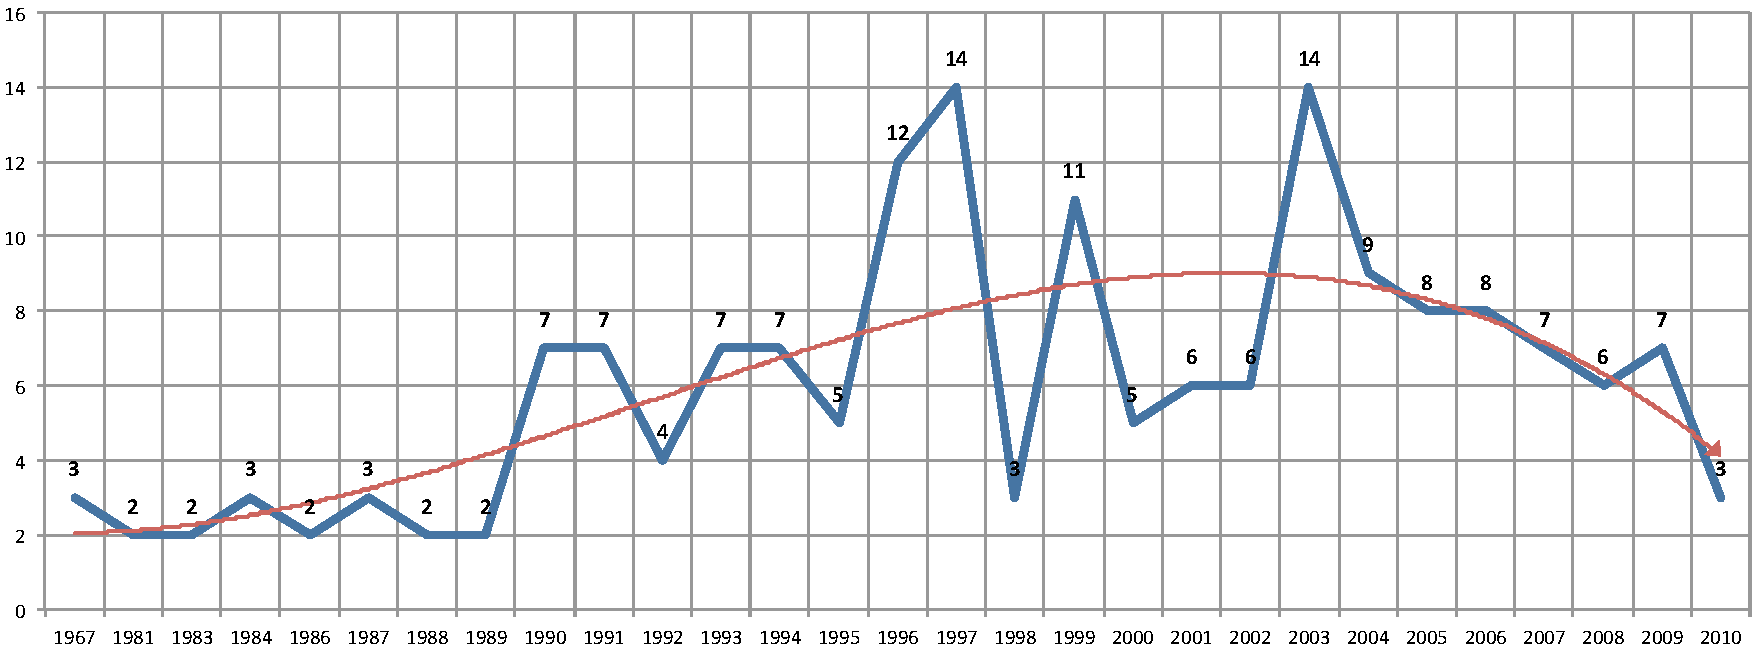
\includegraphics[scale=0.2]{Imagens/abntex2-modelo-img-grafico.pdf}
    \legend{Fonte: \citeonline[p. 24]{araujo2012}}
  \end{minipage}
\end{figure}

Observe que, segundo a \citeonline[seções 4.2.1.10 e 5.8]{NBR14724:2011}, as
ilustrações devem sempre ter numeração contínua e única em todo o documento:

\begin{citacao}
Qualquer que seja o tipo de ilustração, sua identificação aparece na parte
superior, precedida da palavra designativa (desenho, esquema, fluxograma,
fotografia, gráfico, mapa, organograma, planta, quadro, retrato, figura,
imagem, entre outros), seguida de seu número de ordem de ocorrência no texto,
em algarismos arábicos, travessão e do respectivo título. Após a ilustração, na
parte inferior, indicar a fonte consultada (elemento obrigatório, mesmo que
seja produção do próprio autor), legenda, notas e outras informações
necessárias à sua compreensão (se houver). A ilustração deve ser citada no
texto e inserida o mais próximo possível do trecho a que se
refere. \cite[seções 5.8]{NBR14724:2011}
\end{citacao}

% ---
\section{Expressões matemáticas}
% ---

\index{expressões matemáticas}Use o ambiente \texttt{equation} para escrever
expressões matemáticas numeradas:

\begin{equation}
  \forall x \in X, \quad \exists \: y \leq \epsilon
\end{equation}

Escreva expressões matemáticas entre \$ e \$, como em $ \lim_{x \to \infty}
\exp(-x) = 0 $, para que fiquem na mesma linha.

Também é possível usar colchetes para indicar o início de uma expressão
matemática que não é numerada.

\[
\left|\sum_{i=1}^n a_ib_i\right|
\le
\left(\sum_{i=1}^n a_i^2\right)^{1/2}
\left(\sum_{i=1}^n b_i^2\right)^{1/2}
\]

Consulte mais informações sobre expressões matemáticas em
\url{https://github.com/abntex/abntex2/wiki/Referencias}.

% ---
\section{Enumerações: alíneas e subalíneas}
% ---

\index{alíneas}\index{subalíneas}\index{incisos}Quando for necessário enumerar
os diversos assuntos de uma seção que não possua título, esta deve ser
subdividida em alíneas \cite[4.2]{NBR6024:2012}:

\begin{alineas}

  \item os diversos assuntos que não possuam título próprio, dentro de uma mesma
  seção, devem ser subdivididos em alíneas; 
  
  \item o texto que antecede as alíneas termina em dois pontos;
  \item as alíneas devem ser indicadas alfabeticamente, em letra minúscula,
  seguida de parêntese. Utilizam-se letras dobradas, quando esgotadas as
  letras do alfabeto;

  \item as letras indicativas das alíneas devem apresentar recuo em relação à
  margem esquerda;

  \item o texto da alínea deve começar por letra minúscula e terminar em
  ponto-e-vírgula, exceto a última alínea que termina em ponto final;

  \item o texto da alínea deve terminar em dois pontos, se houver subalínea;

  \item a segunda e as seguintes linhas do texto da alínea começa sob a
  primeira letra do texto da própria alínea;
  
  \item subalíneas \cite[4.3]{NBR6024:2012} devem ser conforme as alíneas a
  seguir:

  \begin{alineas}
     \item as subalíneas devem começar por travessão seguido de espaço;

     \item as subalíneas devem apresentar recuo em relação à alínea;

     \item o texto da subalínea deve começar por letra minúscula e terminar em
     ponto-e-vírgula. A última subalínea deve terminar em ponto final, se não
     houver alínea subsequente;

     \item a segunda e as seguintes linhas do texto da subalínea começam sob a
     primeira letra do texto da própria subalínea.
  \end{alineas}
  
  \item no \abnTeX\ estão disponíveis os ambientes \texttt{incisos} e
  \texttt{subalineas}, que em suma são o mesmo que se criar outro nível de
  \texttt{alineas}, como nos exemplos à seguir:
  
  \begin{incisos}
    \item \textit{Um novo inciso em itálico};
  \end{incisos}
  
  \item Alínea em \textbf{negrito}:
  
  \begin{subalineas}
    \item \textit{Uma subalínea em itálico};
    \item \underline{\textit{Uma subalínea em itálico e sublinhado}}; 
  \end{subalineas}
  
  \item Última alínea com \emph{ênfase}.
  
\end{alineas}

% ---
\section{Espaçamento entre parágrafos e linhas}
% ---

\index{espaçamento!dos parágrafos}O tamanho do parágrafo, espaço entre a margem
e o início da frase do parágrafo, é definido por:

\begin{verbatim}
   \setlength{\parindent}{1.3cm}
\end{verbatim}

\index{espaçamento!do primeiro parágrafo}Por padrão, não há espaçamento no
primeiro parágrafo de cada início de divisão do documento
(\autoref{sec-divisoes}). Porém, você pode definir que o primeiro parágrafo
também seja indentado, como é o caso deste documento. Para isso, apenas inclua o
pacote \textsf{indentfirst} no preâmbulo do documento:

\begin{verbatim}
   \usepackage{indentfirst}      % Indenta o primeiro parágrafo de cada seção.
\end{verbatim}

\index{espaçamento!entre os parágrafos}O espaçamento entre um parágrafo e outro
pode ser controlado por meio do comando:

\begin{verbatim}
  \setlength{\parskip}{0.2cm}  % tente também \onelineskip
\end{verbatim}

\index{espaçamento!entre as linhas}O controle do espaçamento entre linhas é
definido por:

\begin{verbatim}
  \OnehalfSpacing       % espaçamento um e meio (padrão); 
  \DoubleSpacing        % espaçamento duplo
  \SingleSpacing        % espaçamento simples	
\end{verbatim}

Para isso, também estão disponíveis os ambientes:

\begin{verbatim}
  \begin{SingleSpace} ...\end{SingleSpace}
  \begin{Spacing}{hfactori} ... \end{Spacing}
  \begin{OnehalfSpace} ... \end{OnehalfSpace}
  \begin{OnehalfSpace*} ... \end{OnehalfSpace*}
  \begin{DoubleSpace} ... \end{DoubleSpace}
  \begin{DoubleSpace*} ... \end{DoubleSpace*} 
\end{verbatim}

Para mais informações, consulte \citeonline[p. 47-52 e 135]{memoir}.

% ---
\section{Inclusão de outros arquivos}\label{sec-include}
% ---

É uma boa prática dividir o seu documento em diversos arquivos, e não
apenas escrever tudo em um único. Esse recurso foi utilizado neste
documento. Para incluir diferentes arquivos em um arquivo principal,
de modo que cada arquivo incluído fique em uma página diferente, utilize o
comando:

\begin{verbatim}
   \include{documento-a-ser-incluido}      % sem a extensão .tex
\end{verbatim}

Para incluir documentos sem quebra de páginas, utilize:

\begin{verbatim}
   \input{documento-a-ser-incluido}      % sem a extensão .tex
\end{verbatim}

% ---
\section{Compilar o documento \LaTeX}
% ---

Geralmente os editores \LaTeX, como o
TeXlipse\footnote{\url{http://texlipse.sourceforge.net/}}, o
Texmaker\footnote{\url{http://www.xm1math.net/texmaker/}}, entre outros,
compilam os documentos automaticamente, de modo que você não precisa se
preocupar com isso.

No entanto, você pode compilar os documentos \LaTeX usando os seguintes
comandos, que devem ser digitados no \emph{Prompt de Comandos} do Windows ou no
\emph{Terminal} do Mac ou do Linux:

\begin{verbatim}
   pdflatex ARQUIVO_PRINCIPAL.tex
   bibtex ARQUIVO_PRINCIPAL.aux
   makeindex ARQUIVO_PRINCIPAL.idx 
   makeindex ARQUIVO_PRINCIPAL.nlo -s nomencl.ist -o ARQUIVO_PRINCIPAL.nls
   pdflatex ARQUIVO_PRINCIPAL.tex
   pdflatex ARQUIVO_PRINCIPAL.tex
\end{verbatim}

% ---
\section{Remissões internas}
% ---

Ao nomear a \autoref{tab-nivinv} e a \autoref{fig_circulo}, apresentamos um
exemplo de remissão interna, que também pode ser feita quando indicamos o
\autoref{cap_exemplos}, que tem o nome \emph{\nameref{cap_exemplos}}. O número
do capítulo indicado é \ref{cap_exemplos}, que se inicia à
\autopageref{cap_exemplos}\footnote{O número da página de uma remissão pode ser
obtida também assim:
\pageref{cap_exemplos}.}.
Veja a \autoref{sec-divisoes} para outros exemplos de remissões internas entre
seções, subseções e subsubseções.

O código usado para produzir o texto desta seção é:

\begin{verbatim}
Ao nomear a \autoref{tab-nivinv} e a \autoref{fig_circulo}, apresentamos um
exemplo de remissão interna, que também pode ser feita quando indicamos o
\autoref{cap_exemplos}, que tem o nome \emph{\nameref{cap_exemplos}}. O número
do capítulo indicado é \ref{cap_exemplos}, que se inicia à
\autopageref{cap_exemplos}\footnote{O número da página de uma remissão pode ser
obtida também assim:
\pageref{cap_exemplos}.}.
Veja a \autoref{sec-divisoes} para outros exemplos de remissões internas entre
seções, subseções e subsubseções.
\end{verbatim}

% ---
\section{Divisões do documento: seção}\label{sec-divisoes}
% ---

Esta seção testa o uso de divisões de documentos. Esta é a
\autoref{sec-divisoes}. Veja a \autoref{sec-divisoes-subsection}.

\subsection{Divisões do documento: subseção}\label{sec-divisoes-subsection}

Isto é uma subseção. Veja a \autoref{sec-divisoes-subsubsection}, que é uma
\texttt{subsubsection} do \LaTeX, mas é impressa chamada de ``subseção'' porque
no Português não temos a palavra ``subsubseção''.

\subsubsection{Divisões do documento: subsubseção}
\label{sec-divisoes-subsubsection}

Isto é uma subsubseção.

\subsubsection{Divisões do documento: subsubseção}

Isto é outra subsubseção.

\subsection{Divisões do documento: subseção}\label{sec-exemplo-subsec}

Isto é uma subseção.

\subsubsection{Divisões do documento: subsubseção}

Isto é mais uma subsubseção da \autoref{sec-exemplo-subsec}.


\subsubsubsection{Esta é uma subseção de quinto
nível}\label{sec-exemplo-subsubsubsection}

Esta é uma seção de quinto nível. Ela é produzida com o seguinte comando:

\begin{verbatim}
\subsubsubsection{Esta é uma subseção de quinto
nível}\label{sec-exemplo-subsubsubsection}
\end{verbatim}

\subsubsubsection{Esta é outra subseção de quinto nível}\label{sec-exemplo-subsubsubsection-outro}

Esta é outra seção de quinto nível.


\paragraph{Este é um parágrafo numerado}\label{sec-exemplo-paragrafo}

Este é um exemplo de parágrafo nomeado. Ele é produzida com o comando de
parágrafo:

\begin{verbatim}
\paragraph{Este é um parágrafo nomeado}\label{sec-exemplo-paragrafo}
\end{verbatim}

A numeração entre parágrafos numeradaos e subsubsubseções são contínuas.

\paragraph{Esta é outro parágrafo numerado}\label{sec-exemplo-paragrafo-outro}

Esta é outro parágrafo nomeado.

% ---
\section{Este é um exemplo de nome de seção longo. Ele deve estar
alinhado à esquerda e a segunda e demais linhas devem iniciar logo abaixo da
primeira palavra da primeira linha}
% ---

Isso atende à norma \citeonline[seções de 5.2.2 a 5.2.4]{NBR14724:2011} 
 e \citeonline[seções de 3.1 a 3.8]{NBR6024:2012}.

% ---
\section{Diferentes idiomas e hifenizações}
\label{sec-hifenizacao}
% ---

Para usar hifenizações de diferentes idiomas, inclua nas opções do documento o
nome dos idiomas que o seu texto contém. Por exemplo (para melhor
visualização, as opções foram quebras em diferentes linhas):

\begin{verbatim}
\documentclass[
	12pt,
	openright,
	twoside,
	a4paper,
	english,
	french,
	spanish,
	brazil
	]{abntex2}
\end{verbatim}

O idioma português-brasileiro (\texttt{brazil}) é incluído automaticamente pela
classe \textsf{abntex2}. Porém, mesmo assim a opção \texttt{brazil} deve ser
informada como a última opção da classe para que todos os pacotes reconheçam o
idioma. Vale ressaltar que a última opção de idioma é a utilizada por padrão no
documento. Desse modo, caso deseje escrever um texto em inglês que tenha
citações em português e em francês, você deveria usar o preâmbulo como abaixo:

\begin{verbatim}
\documentclass[
	12pt,
	openright,
	twoside,
	a4paper,
	french,
	brazil,
	english
	]{abntex2}
\end{verbatim}

A lista completa de idiomas suportados, bem como outras opções de hifenização,
estão disponíveis em \citeonline[p.~5-6]{babel}.

Exemplo de hifenização em inglês\footnote{Extraído de:
\url{http://en.wikibooks.org/wiki/LaTeX/Internationalization}}:

\begin{otherlanguage*}{english}
\textit{Text in English language. This environment switches all language-related
definitions, like the language specific names for figures, tables etc. to the other
language. The starred version of this environment typesets the main text
according to the rules of the other language, but keeps the language specific
string for ancillary things like figures, in the main language of the document.
The environment hyphenrules switches only the hyphenation patterns used; it can
also be used to disallow hyphenation by using the language name
`nohyphenation'.}
\end{otherlanguage*}

O idioma geral do texto por ser alterado como no exemplo seguinte:

\begin{verbatim}
  \selectlanguage{english}
\end{verbatim}

Isso altera automaticamente a hifenização e todos os nomes constantes de
referências do documento para o idioma inglês. Consulte o manual da classe
\cite{abntex2classe} para obter orientações adicionais sobre internacionalização de
documentos produzidos com \abnTeX.

A \autoref{sec-citacao} descreve o ambiente \texttt{citacao} que pode receber
como parâmetro um idioma a ser usado na citação.

% ---
\section{Consulte o manual da classe \textsf{abntex2}}
% ---

Consulte o manual da classe \textsf{abntex2} \cite{abntex2classe} para uma
referência completa das macros e ambientes disponíveis. 

Além disso, o manual possui informações adicionais sobre as normas ABNT
observadas pelo \abnTeX\ e considerações sobre eventuais requisitos específicos
não atendidos, como o caso da \citeonline[seção 5.2.2]{NBR14724:2011}, que
especifica o espaçamento entre os capítulos e o início do texto, regra
propositalmente não atendida pelo presente modelo.

% ---
\section{Referências bibliográficas}
% ---

A formatação das referências bibliográficas conforme as regras da ABNT são um
dos principais objetivos do \abnTeX. Consulte os manuais
\citeonline{abntex2cite} e \citeonline{abntex2cite-alf} para obter informações
sobre como utilizar as referências bibliográficas.

%-
\subsection{Acentuação de referências bibliográficas}
%-

Normalmente não há problemas em usar caracteres acentuados em arquivos
bibliográficos (\texttt{*.bib}). Porém, como as regras da ABNT fazem uso quase
abusivo da conversão para letras maiúsculas, é preciso observar o modo como se
escreve os nomes dos autores. Na ~\autoref{tabela-acentos} você encontra alguns
exemplos das conversões mais importantes. Preste atenção especial para `ç' e `í'
que devem estar envoltos em chaves. A regra geral é sempre usar a acentuação
neste modo quando houver conversão para letras maiúsculas.

\begin{table}[htbp]
\caption{Tabela de conversão de acentuação.}
\label{tabela-acentos}

\begin{center}
\begin{tabular}{ll}\hline\hline
acento & \textsf{bibtex}\\
à á ã & \verb+\`a+ \verb+\'a+ \verb+\~a+\\
í & \verb+{\'\i}+\\
ç & \verb+{\c c}+\\
\hline\hline
\end{tabular}
\end{center}
\end{table}


% ---
\section{Precisa de ajuda?}
% ---

Consulte a FAQ com perguntas frequentes e comuns no portal do \abnTeX:
\url{https://github.com/abntex/abntex2/wiki/FAQ}.

Inscreva-se no grupo de usuários \LaTeX:
\url{http://groups.google.com/group/latex-br}, tire suas dúvidas e ajude
outros usuários.

Participe também do grupo de desenvolvedores do \abnTeX:
\url{http://groups.google.com/group/abntex2} e faça sua contribuição à
ferramenta.

% ---
\section{Você pode ajudar?}
% ---

Sua contribuição é muito importante! Você pode ajudar na divulgação, no
desenvolvimento e de várias outras formas. Veja como contribuir com o \abnTeX\
em \url{https://github.com/abntex/abntex2/wiki/Como-Contribuir}.

% ---
\section{Quer customizar os modelos do \abnTeX\ para sua instituição ou universidade?}
% ---

Veja como customizar o \abnTeX\ em: \\
\url{https://github.com/abntex/abntex2/wiki/ComoCustomizar}.
\chapter{Conteúdos específicos do modelo de trabalho acadêmico}\label{cap_trabalho_academico}

\section{Quadros}

Este modelo vem com o ambiente \texttt{quadro} e impressão de Lista de quadros 
configurados por padrão. Verifique um exemplo de utilização:

\begin{quadro}[htb]
\caption{\label{quadro_exemplo}Exemplo de quadro}
\begin{tabular}{|c|c|c|c|}
	\hline
	\textbf{Pessoa} & \textbf{Idade} & \textbf{Peso} & \textbf{Altura} \\ \hline
	Marcos & 26    & 68   & 178    \\ \hline
	Ivone  & 22    & 57   & 162    \\ \hline
	...    & ...   & ...  & ...    \\ \hline
	Sueli  & 40    & 65   & 153    \\ \hline
\end{tabular}
\fonte{Autor.}
\end{quadro}

Este parágrafo apresenta como referenciar o quadro no texto, requisito
obrigatório da ABNT. 
Primeira opção, utilizando \texttt{autoref}: Ver o \autoref{quadro_exemplo}. 
Segunda opção, utilizando  \texttt{ref}: Ver o Quadro \ref{quadro_exemplo}.
% ---
% Capitulo de revisão de literatura
% ---
\chapter{Lorem ipsum dolor sit amet}
% ---

% ---
\section{Aliquam vestibulum fringilla lorem}
% ---

\lipsum[1]

\lipsum[2-3]

% ---
% primeiro capitulo de Resultados
% ---
\chapter{Lectus lobortis condimentum}
% ---

% ---
\section{Vestibulum ante ipsum primis in faucibus orci luctus et ultrices
posuere cubilia Curae}
% ---

\lipsum[21-22]

% ---
% segundo capitulo de Resultados
% ---
\chapter{Nam sed tellus sit amet lectus urna ullamcorper tristique interdum
elementum}
% ---

% ---
\section{Pellentesque sit amet pede ac sem eleifend consectetuer}
% ---

\lipsum[24]
\chapter{Customização DCOMP}

\section{Estratégias em um Novo Paradigma Globalizado}
Por conseguinte, a contínua expansão de nossa atividade apresenta tendências no sentido de aprovar a manutenção das posturas dos órgãos dirigentes com relação às suas atribuições. Por outro lado, a hegemonia do ambiente político exige a precisão e a definição do impacto na agilidade decisória. No mundo atual, o desafiador cenário globalizado facilita a criação das direções preferenciais no sentido do progresso. No entanto, não podemos esquecer que o entendimento das metas propostas estende o alcance e a importância das condições financeiras e administrativas exigidas. Pensando mais a longo prazo, a valorização de fatores subjetivos garante a contribuição de um grupo importante na determinação das regras de conduta normativas, como exemplo o Códigos \ref{labelJava} e o Código \ref{labelPython}.

\begin{listing}[h]
    \caption{Primeiro código C}
    \label{labelJava}
    
    \begin{minted}{c}
    int main() {
        printf("hello world");
        return 0;
    }
    \end{minted}
    
\end{listing}

\begin{listing}[h]
    \caption{Primeiro código Python}
    \label{labelPython}
	\begin{minted}{python}
import numpy as np
 
def incmatrix(genl1,genl2):
    m = len(genl1)
    n = len(genl2)
    M = None #to become the incidence matrix
    VT = np.zeros((n*m,1), int)  #dummy variable
 
    #compute the bitwise xor matrix
    M1 = bitxormatrix(genl1)
    M2 = np.triu(bitxormatrix(genl2),1) 
 
    for i in range(m-1):
        for j in range(i+1, m):
            [r,c] = np.where(M2 == M1[i,j])
            for k in range(len(r)):
                VT[(i)*n + r[k]] = 1;
                VT[(i)*n + c[k]] = 1;
                VT[(j)*n + r[k]] = 1;
                VT[(j)*n + c[k]] = 1;
 
                if M is None:
                    M = np.copy(VT)
                else:
                    M = np.concatenate((M, VT), 1)
 
                VT = np.zeros((n*m,1), int)
 
    return M
	\end{minted}
\end{listing}

É importante questionar o quanto a adoção de políticas descentralizadoras desafia a capacidade de equalização dos índices pretendidos. Neste sentido, a constante divulgação das informações promove a alavancagem do processo de comunicação como um todo. As experiências acumuladas demonstram que a consolidação das estruturas obstaculiza a apreciação da importância dos níveis de motivação departamental. Acima de tudo, é fundamental ressaltar que a consulta aos diversos militantes oferece uma interessante oportunidade para verificação das condições inegavelmente apropriadas. A prática cotidiana prova que o início da atividade geral de formação de atitudes acarreta um processo de reformulação e modernização do retorno esperado a longo prazo. 

Não obstante, o novo modelo estrutural aqui preconizado prepara-nos para enfrentar situações atípicas decorrentes dos paradigmas corporativos. Gostaria de enfatizar que a mobilidade dos capitais internacionais afeta positivamente a correta previsão das novas proposições. O que temos que ter sempre em mente é que o desenvolvimento contínuo de distintas formas de atuação representa uma abertura para a melhoria do investimento em reciclagem técnica. Ainda assim, existem dúvidas a respeito de como a necessidade de renovação processual talvez venha a ressaltar a relatividade dos métodos utilizados na avaliação de resultados. 

Nunca é demais lembrar o peso e o significado destes problemas, uma vez que o consenso sobre a necessidade de qualificação aponta para a melhoria do remanejamento dos quadros funcionais. A nível organizacional, o surgimento do comércio virtual maximiza as possibilidades por conta do sistema de participação geral. O empenho em analisar a crescente influência da mídia possibilita uma melhor visão global do orçamento setorial. 

Assim mesmo, a competitividade nas transações comerciais auxilia a preparação e a composição dos modos de operação convencionais. O cuidado em identificar pontos críticos no comprometimento entre as equipes é uma das consequências de alternativas às soluções ortodoxas. Percebemos, cada vez mais, que a estrutura atual da organização nos obriga à análise dos procedimentos normalmente adotados. Todavia, o julgamento imparcial das eventualidades pode nos levar a considerar a reestruturação do sistema de formação de quadros que corresponde às necessidades.
\chapter{Conclusão}

\lipsum

\phantompart
\bibliography{Bibliografia}

% ----------------------------------------------------------
% ELEMENTOS PÓS-TEXTUAIS
% ----------------------------------------------------------
\postextual

\renewcommand{\chapnumfont}{\chaptitlefont}
\renewcommand{\afterchapternum}{}
\begin{apendicesenv}

% Imprime uma página indicando o início dos apêndices
\partapendices

% ----------------------------------------------------------
\chapter{Quisque libero justo}
% ----------------------------------------------------------

\lipsum[50]

% ----------------------------------------------------------
\chapter{Nullam elementum urna vel imperdiet sodales elit ipsum pharetra ligula
ac pretium ante justo a nulla curabitur tristique arcu eu metus}
% ----------------------------------------------------------
\lipsum[55-57]

\end{apendicesenv}

\begin{anexosenv}


% Imprime uma página indicando o início dos anexos
\partanexos

% ---
\chapter{Morbi ultrices rutrum lorem.}
% ---
\lipsum[30]

% ---
\chapter{Cras non urna sed feugiat cum sociis natoque penatibus et magnis dis
parturient montes nascetur ridiculus mus}
% ---

\lipsum[31]

% ---
\chapter{Fusce facilisis lacinia dui}
% ---

\lipsum[32]


\end{anexosenv}


\end{document}